\documentclass[fleqn]{article}

\usepackage{graphicx}
\usepackage{xurl}
\usepackage{url}
\usepackage{caption}
\usepackage{fancyhdr}
\usepackage{mathtools}
\usepackage{amsmath}
\usepackage{amssymb}
\usepackage{tikz}
\usepackage{listings}
\usepackage{xcolor}
\usepackage{float}

\definecolor{codegreen}{rgb}{0,0.6,0}
\definecolor{codegray}{rgb}{0.5,0.5,0.5}
\definecolor{codepurple}{rgb}{0.58,0,0.82}
\definecolor{backcolour}{rgb}{0.95,0.95,0.92}

\lstdefinestyle{mystyle}{
	backgroundcolor=\color{backcolour},   
	commentstyle=\color{codegreen},
	keywordstyle=\color{magenta},
	numberstyle=\tiny\color{codegray},
	stringstyle=\color{codepurple},
	basicstyle=\ttfamily\footnotesize,
	breakatwhitespace=false,         
	breaklines=true,                 
	captionpos=b,                    
	keepspaces=true,                 
	numbers=left,                    
	numbersep=5pt,                  
	showspaces=false,                
	showstringspaces=false,
	showtabs=false,                  
	tabsize=2
}

\lstset{style=mystyle}

\usepackage{xepersian}

\settextfont[BoldFont={XB Zar bold.ttf}]{XB Zar.ttf}
\setlength\parindent{0pt}

\title{

\includegraphics[width=0.4\textwidth]{sharif.png}\\
\normalsize{دانشکده مهندسی کامپیوتر}\\
\vspace{1cm}
	
\huge{آزمایشگاه طراحی سیستم‌های دیجیتال}
\\
\Large{گزارش آزمایش سوم}
\\
}

\author{
\\
دکتر سیاوش بیات سرمدی
\\
\\
پارسا محمدیان --- 98102284
}

\date{\today}

\begin{document}

\clearpage\maketitle
\thispagestyle{empty}

\newpage

\pagestyle{fancy}
\lhead{آزمایشگاه طراحی سیستم‌های دیجیتال}

\rhead{پارسا محمدیان}


\tableofcontents

\setcounter{page}{1}

\newpage

\section{مقدمه}

\subsection*{عنوان گزارش}
توصیف جریان داده
\subsection*{موضوع}
استفاده از نرم‌افزارهای طراحی به کمک کامپیوتر \footnote{\lr{CAD}} برای طراحی 
و پیاده‌سازی مدار ترکیبی و ترتیبی به صورت جریان داده.
\subsection*{شرح ابزارها و برنامه‌های مورد استفاده}
در این آزمایش از نرم‌افزار \lr{ISE Desgin Suite} که محصول شرکت \lr{Xilinx} است 
استفاده کرده‌ام.

\section{چارچوب نظری و شرح آزمایش}
\subsection{بخش اول}
در بخش اول آزمایش با استفاده از توصیف جریان داده یک مقایسه کننده یک بیتی 
ساختیم
\\(\lr{OneBitComparator.v}).
\\
 سپس با گرفتن 4 نمونه از ماژول مورد نظر، یک 
مقایسه کننده 4 بیتی ساختیم که ورودی آن به صورت پارالل 
است(\lr{FourBitComparator.v}).

\subsection{بخش دوم}
برای انجام بخش دوم، چون مدار ترتیبی است، نیاز به یک حافظه داریم. در اینجا 
از \lr{D Flip-Flop} استفاده کرده‌ام که شماتیک آن در شکل \ref{dff} آمده است.

\begin{figure}[!htbp]
	\centering
	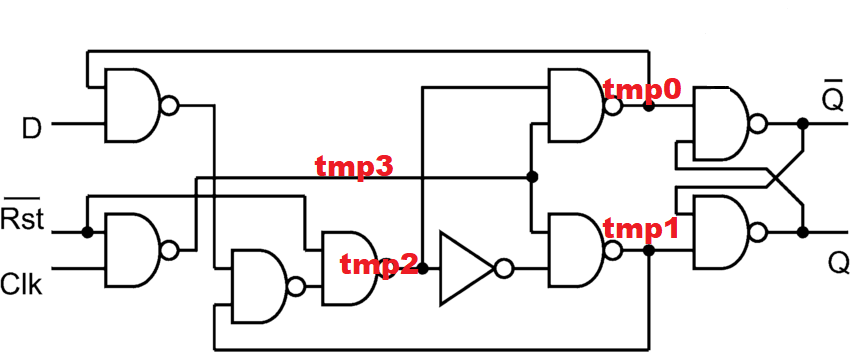
\includegraphics[width=.5\paperwidth]{dff.png}
	\caption{شماتیک فلیپ فلاپ نوع \lr{D}}
	\label{dff}
\end{figure}

این فلیپ فلاپ باید به صورت جریان داده پیاده سازی شود. همچنین مابقی جزئیات 
پیاده سازی نیز در فایل \lr{SerialComparator.v} موجود است.

\section{گزارش متنی بخش \lr{Place \& Route}}
گزارش متنی بخش \lr{Place \& Route} برای ماژول \lr{FourBitComparator} در ادامه 
آمده است.
\begin{latin}
\begin{lstlisting}[basicstyle=\tiny]
Release 14.7 par P.20131013 (nt64)
Copyright (c) 1995-2013 Xilinx, Inc.  All rights reserved.

DESKTOP-PRL8LS0::  Wed Apr 14 11:58:24 2021

par -w -intstyle ise -ol high -t 1 FourBitComparator_map.ncd
FourBitComparator.ncd FourBitComparator.pcf 


Constraints file: FourBitComparator.pcf.
Loading device for application Rf_Device from file '3sd3400a.nph' in 
environment C:\Xilinx\14.7\ISE_DS\ISE\.
"FourBitComparator" is an NCD, version 3.2, device xc3sd3400a, package fg676, 
speed -4

Initializing temperature to 85.000 Celsius. (default - Range: 0.000 to 85.000 
Celsius)
Initializing voltage to 1.140 Volts. (default - Range: 1.140 to 1.260 Volts)

INFO:Par:282 - No user timing constraints were detected or you have set the 
option to ignore timing constraints ("par
-x"). Place and Route will run in "Performance Evaluation Mode" to 
automatically improve the performance of all
internal clocks in this design. Because there are not defined timing 
requirements, a timing score will not be
reported in the PAR report in this mode. The PAR timing summary will list the 
performance achieved for each clock.
Note: For the fastest runtime, set the effort level to "std".  For best 
performance, set the effort level to "high".

Device speed data version:  "PRODUCTION 1.34 2013-10-13".


Design Summary Report:

Number of External IOBs                          11 out of 469     2%

Number of External Input IOBs                  8

Number of External Input IBUFs              8

Number of External Output IOBs                 3

Number of External Output IOBs              3

Number of External Bidir IOBs                  0


Number of Slices                          4 out of 23872   1%
Number of SLICEMs                      0 out of 11936   0%



Overall effort level (-ol):   High 
Placer effort level (-pl):    High 
Placer cost table entry (-t): 1
Router effort level (-rl):    High 

Starting initial Timing Analysis.  REAL time: 2 secs 
Finished initial Timing Analysis.  REAL time: 2 secs 


Starting Placer
Total REAL time at the beginning of Placer: 2 secs 
Total CPU  time at the beginning of Placer: 2 secs 

Phase 1.1  Initial Placement Analysis
Phase 1.1  Initial Placement Analysis (Checksum:6e) REAL time: 3 secs 

Phase 2.7  Design Feasibility Check
Phase 2.7  Design Feasibility Check (Checksum:6e) REAL time: 3 secs 

Phase 3.31  Local Placement Optimization
Phase 3.31  Local Placement Optimization (Checksum:6e) REAL time: 3 secs 

Phase 4.2  Initial Clock and IO Placement
..........
Phase 4.2  Initial Clock and IO Placement (Checksum:6e) REAL time: 3 secs 

Phase 5.30  Global Clock Region Assignment
Phase 5.30  Global Clock Region Assignment (Checksum:6e) REAL time: 3 secs 

Phase 6.36  Local Placement Optimization
Phase 6.36  Local Placement Optimization (Checksum:6e) REAL time: 3 secs 

Phase 7.3  Local Placement Optimization
...........
Phase 7.3  Local Placement Optimization (Checksum:357b0a) REAL time: 3 secs 

Phase 8.5  Local Placement Optimization
Phase 8.5  Local Placement Optimization (Checksum:357b0a) REAL time: 3 secs 

Phase 9.8  Global Placement
..
Phase 9.8  Global Placement (Checksum:19a336a) REAL time: 3 secs 

Phase 10.5  Local Placement Optimization
Phase 10.5  Local Placement Optimization (Checksum:19a336a) REAL time: 3 secs 

Phase 11.18  Placement Optimization
Phase 11.18  Placement Optimization (Checksum:2171395) REAL time: 4 secs 

Phase 12.5  Local Placement Optimization
Phase 12.5  Local Placement Optimization (Checksum:2171395) REAL time: 4 secs 

Total REAL time to Placer completion: 4 secs 
Total CPU  time to Placer completion: 3 secs 
Writing design to file FourBitComparator.ncd



Starting Router


Phase  1  : 29 unrouted;      REAL time: 20 secs 

Phase  2  : 29 unrouted;      REAL time: 20 secs 

Phase  3  : 6 unrouted;      REAL time: 20 secs 

Phase  4  : 6 unrouted; (Par is working to improve performance)     REAL time: 
22 secs 

Phase  5  : 0 unrouted; (Par is working to improve performance)     REAL time: 
22 secs 

Updating file: FourBitComparator.ncd with current fully routed design.

Phase  6  : 0 unrouted; (Par is working to improve performance)     REAL time: 
22 secs 

Phase  7  : 0 unrouted; (Par is working to improve performance)     REAL time: 
22 secs 

Phase  8  : 0 unrouted; (Par is working to improve performance)     REAL time: 
22 secs 

Phase  9  : 0 unrouted; (Par is working to improve performance)     REAL time: 
22 secs 

Total REAL time to Router completion: 22 secs 
Total CPU time to Router completion: 22 secs 

Partition Implementation Status
-------------------------------

No Partitions were found in this design.

-------------------------------

Generating "PAR" statistics.

Timing Score: 0 (Setup: 0, Hold: 0)



Generating Pad Report.

All signals are completely routed.

Total REAL time to PAR completion: 23 secs 
Total CPU time to PAR completion: 23 secs 

Peak Memory Usage:  4578 MB

Placement: Completed - No errors found.
Routing: Completed - No errors found.

Number of error messages: 0
Number of warning messages: 0
Number of info messages: 1

Writing design to file FourBitComparator.ncd



PAR done!
\end{lstlisting}
\end{latin}


از \lr{Text Report} اطلاعات زیر بدست می‌آید. با توجه به اینکه کد را به صورت 
جریان داده زده‌ایم، تعداد رجیسترها و \lr{LUT} ها وجود ندارد.
\begin{latin}
\begin{verbatim}
	Number of Slices                          4 out of 23872   1%
	   Number of SLICEMs                      0 out of 11936   0%
\end{verbatim}
\end{latin}

\section{تست مدار}
برای تست بخش اول، دو تست بنچ در فایل‌های 
\\\lr{FourBitComparatorTest.v} و 
\lr{OneBitComparatorTest.v} می‌نویسیم.

برای تست بخش دوم نیز تست بنچ در فایل \lr{SerialComparatorTest.v} موجود است.
\end{document}
